\documentclass[12pt, A4]{article}
\usepackage[utf8]{inputenc}
\usepackage{graphicx}
\usepackage[margin=0.5in]{geometry}
\usepackage{hyperref}

\title{Lab 1 Report}
\author{Anton Gashi: 201914462}
\date

\begin{document}

\begin{titlepage}
\clearpage\maketitle
\thispagestyle{empty}
\end{titlepage}

\section*{\underline{Task 1}}
\hspace{1.5em}\textbf{Task From Lab Sheet:} \\ \\ Using different initial seeds and at least two different pseudo-random generators, produce sequences of uniformly distributed random numbers. Test these values for a) uniformity and b) lack of sequential correlation. Present your analysis as graphically as possible.

\vspace{1.5em}

\textbf{My Result:} \\ \\ The two different pseudo-random generators I used were \href{https://numpy.org/doc/stable/reference/random/generated/numpy.random.uniform.html}{numpy.random.uniform} and \href{https://numpy.org/doc/stable/reference/random/generated/numpy.random.choice.html}{numpy.random.choice}. \\ The Chi squared for the uniform distribution is $\chi_{uniform}$ = 89.42 ($\le$ 100) and $\chi_{choice}$ = 158.36 for the random choice distribution, the reason for the larger Chi squared value for the second generator is due to the fact that the choice is made from the first generator \textbf{with} replacement. If 'replace=False' then the Chi squared becomes the exact same as the first.


\begin{center}
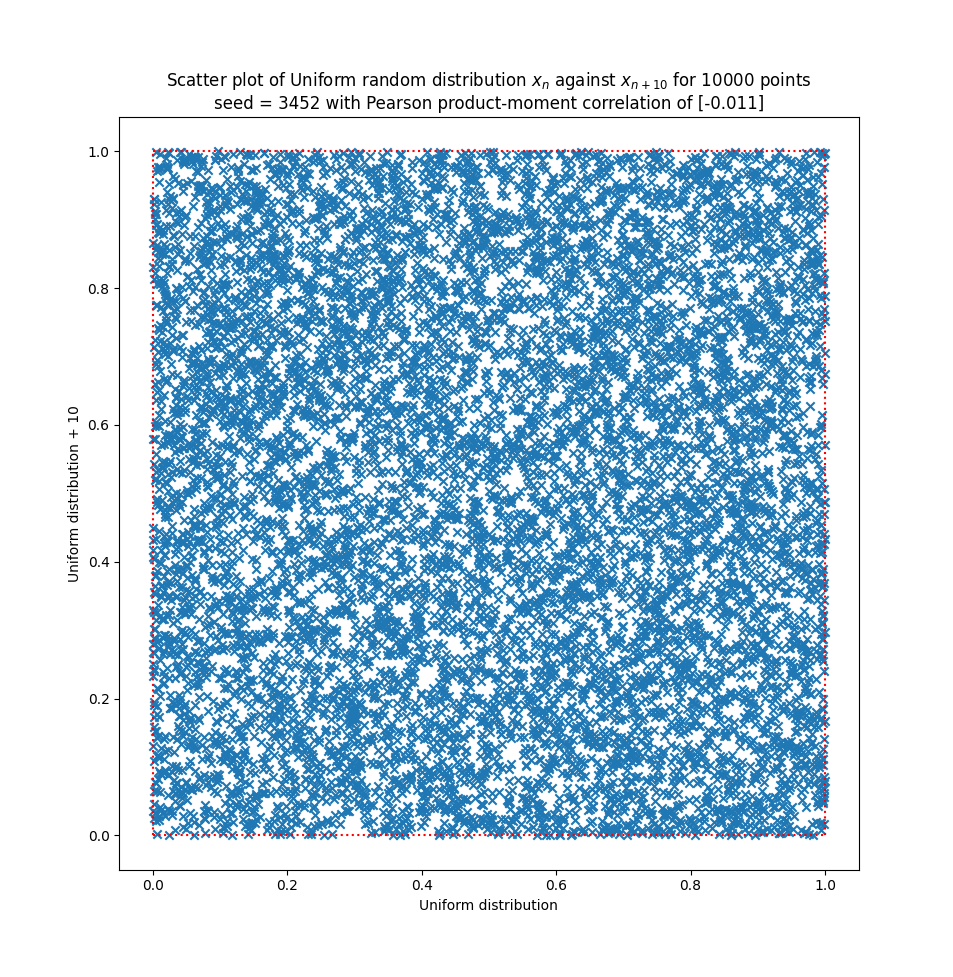
\includegraphics[scale=0.35]{Task_1_Scatter}
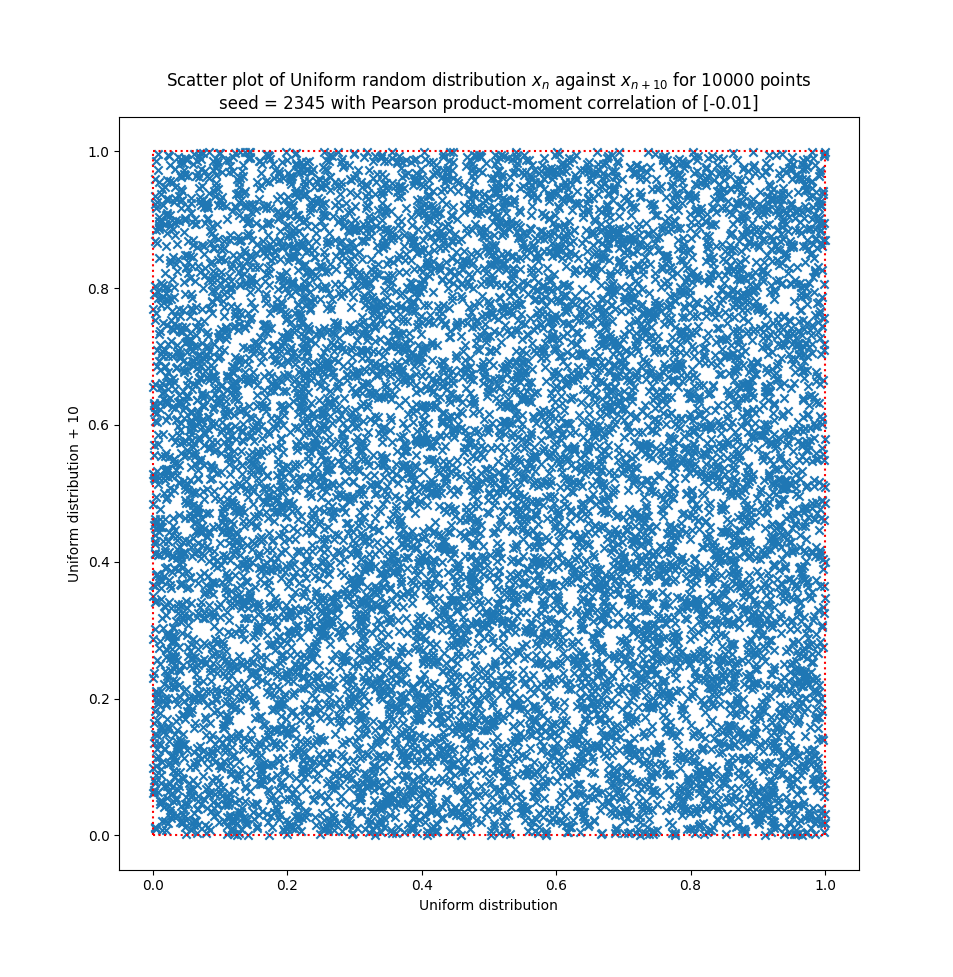
\includegraphics[scale=0.35]{Task_1_Scatter1}
\end{center}


\section*{\underline{Task 2}}
\hspace{1.5em}\textbf{Task From Lab Sheet:} \\ \\ Write a program to simulate a partitioned box containing N particles, initially all on one side of the partition, with an equal probability of any one particle moving from one side of the partition to the other in unit time. Present your results graphically as well as textually.

\vspace{1.5em}

\textbf{My Result:} \\ \\ 

\begin{center}
	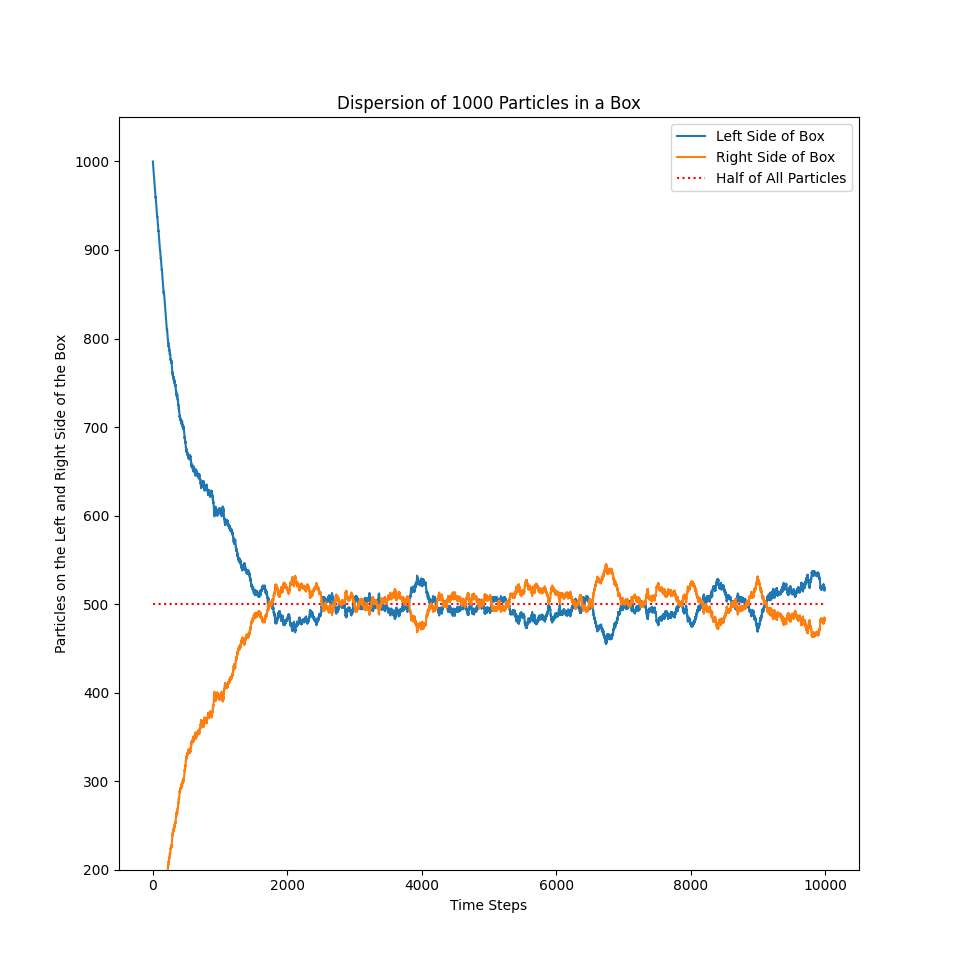
\includegraphics[scale=0.5]{Task_2_Line}
\end{center}

\section*{\underline{Task 3}}

\section*{\underline{Task 4}}

\end{document}
